\documentclass[portrate,paperwidth=841mm,paperheight=1189mm,fontscale=0.4,margin=1cm]{baposter}
%\documentclass[landscape,paperwidth=1682mm,paperheight=1189mm,fontscale=0.4,margin=3cm]{baposter}

\usepackage{calc}
\usepackage{graphicx}
\usepackage{amsmath}
\usepackage{amssymb}
\usepackage{relsize}
\usepackage{multirow}
\usepackage{rotating}
\usepackage{bm}
\usepackage{enumitem}
\usepackage{booktabs}
\usepackage{relsize}		% For \smaller
\usepackage{url}			% For \url

\usepackage{graphicx}
\usepackage{multicol}
\usepackage{wrapfig}
%\usepackage{times}
%\usepackage{helvet}
%\usepackage{bookman}
\usepackage{palatino}
%% Pablo's personal packages
%% AMS unofficial LateX proceeding template:
%%    http://www.cimms.ou.edu/~lakshman/ametsoc/
%%\usepackage[hypertex]{hyperref}
%% end personal packages

\newcommand{\captionfont}{\footnotesize}

\graphicspath{{images/}{./images}}
\usetikzlibrary{calc}


\newcommand{\Matrix}[1]{\begin{bmatrix} #1 \end{bmatrix}}
\newcommand{\Vector}[1]{\begin{pmatrix} #1 \end{pmatrix}}

\newcommand*{\norm}[1]{\mathopen\| #1 \mathclose\|}% use instead of $\|x\|$
\newcommand*{\abs}[1]{\mathopen| #1 \mathclose|}% use instead of $\|x\|$
\newcommand*{\normLR}[1]{\left\| #1 \right\|}% use instead of $\|x\|$

\newcommand*{\SET}[1]  {\ensuremath{\mathcal{#1}}}
\newcommand*{\FUN}[1]  {\ensuremath{\mathcal{#1}}}
\newcommand*{\MAT}[1]  {\ensuremath{\boldsymbol{#1}}}
\newcommand*{\VEC}[1]  {\ensuremath{\boldsymbol{#1}}}
\newcommand*{\CONST}[1]{\ensuremath{\mathit{#1}}}

\DeclareMathOperator*{\argmax}{arg\,max}
\DeclareMathOperator*{\diag}{diag}
\DeclareMathOperator*{\argmin}{arg\,min}
\DeclareMathOperator*{\vectorize}{vec}
\DeclareMathOperator*{\reshape}{reshape}

%\font\dsfnt=dsrom12

\newcommand{\SNN}{\ensuremath{\mathbb N}}
\newcommand{\SRR}{\ensuremath{\mathbb R}}
\newcommand{\SZZ}{\ensuremath{\mathbb Z}}
%-----------------------------------------------------------------------------
% Matrices of the shape model
\renewcommand{\a}{\VEC\alpha}
\renewcommand{\v}{\VEC v}
\renewcommand{\l}{\VEC l}
\newcommand*{\m}{\VEC{\mu}}
\newcommand*{\M}{\MAT{M}}
\renewcommand*{\P}{\MAT{\Pi}}

%\newcommand{\J}{\SET J}
\newcommand{\J}{\SET{P}}
\newcommand{\Active}{\mathcal{A}}
\newcommand{\Selection}{\mathbf{S}}
\newcommand{\AllSelections}{\mathfrak{S}}
\newcommand{\Params}{\VEC\Theta}

%%%%%%%%%%%%%%%%%%%%%%%%%%%%%%%%%%%%%%%%%%%%%%%%%%%%%%%%%%%%%%%%%%%%%%%%%%%%%%%%
%%%% Some math symbols used in the text
%%%%%%%%%%%%%%%%%%%%%%%%%%%%%%%%%%%%%%%%%%%%%%%%%%%%%%%%%%%%%%%%%%%%%%%%%%%%%%%%

%%%%%%%%%%%%%%%%%%%%%%%%%%%%%%%%%%%%%%%%%%%%%%%%%%%%%%%%%%%%%%%%%%%%%%%%%%%%%%%%
% Multicol Settings
%%%%%%%%%%%%%%%%%%%%%%%%%%%%%%%%%%%%%%%%%%%%%%%%%%%%%%%%%%%%%%%%%%%%%%%%%%%%%%%%
\setlength{\columnsep}{1.5em}
\setlength{\columnseprule}{0mm}

%%%%%%%%%%%%%%%%%%%%%%%%%%%%%%%%%%%%%%%%%%%%%%%%%%%%%%%%%%%%%%%%%%%%%%%%%%%%%%%%
% Save space in lists. Use this after the opening of the list
%%%%%%%%%%%%%%%%%%%%%%%%%%%%%%%%%%%%%%%%%%%%%%%%%%%%%%%%%%%%%%%%%%%%%%%%%%%%%%%%
\newcommand{\compresslist}{%
\setlength{\itemsep}{1pt}%
\setlength{\parskip}{0pt}%
\setlength{\parsep}{0pt}%
}

%%%%%%%%%%%%%%%%%%%%%%%%%%%%%%%%%%%%%%%%%%%%%%%%%%%%%%%%%%%%%%%%%%%%%%%%%%%%%%
%%% Begin of Document
%%%%%%%%%%%%%%%%%%%%%%%%%%%%%%%%%%%%%%%%%%%%%%%%%%%%%%%%%%%%%%%%%%%%%%%%%%%%%%

\begin{document}

%%%%%%%%%%%%%%%%%%%%%%%%%%%%%%%%%%%%%%%%%%%%%%%%%%%%%%%%%%%%%%%%%%%%%%%%%%%%%%
%%% Here starts the poster
%%%---------------------------------------------------------------------------
%%% Format it to your taste with the options
%%%%%%%%%%%%%%%%%%%%%%%%%%%%%%%%%%%%%%%%%%%%%%%%%%%%%%%%%%%%%%%%%%%%%%%%%%%%%%
% Define some colors

\definecolor{silver}{cmyk}{0,0,0,0.3}
\definecolor{yellow}{cmyk}{0,0,0.9,0.0}
\definecolor{reddishyellow}{cmyk}{0,0.22,1.0,0.0}
\definecolor{black}{cmyk}{0,0,0.0,1.0}
\definecolor{white}{rgb}{1,1,1}
\definecolor{red}{rgb}{.9,0,0}
\definecolor{green}{rgb}{0,.3,0}
\definecolor{blue}{rgb}{.21,.24,.36}

\definecolor{darkYellow}{cmyk}{0,0,1.0,0.5}
\definecolor{darkSilver}{cmyk}{0,0,0,0.1}

\definecolor{middlegray}{rgb}{.4,.4,.4}
\definecolor{lightgray}{rgb}{.7,.7,.7}

\definecolor{lightgreen}{rgb}{.7,7,.35}
\definecolor{lightlila}{rgb}{.6,.6,.8}
\definecolor{lightorange}{rgb}{.88,.74,.15}
\definecolor{lighterorange}{rgb}{.98,.84,.45}
\definecolor{middleblue}{rgb}{.447,.537,.9513}
\definecolor{lightblue}{rgb}{.447,.537,.6313}
\definecolor{lighterblue}{rgb}{.568,.639,.709}
\definecolor{lighteryellow}{cmyk}{0,0,0.1,0.0}
\definecolor{lightestblue}{rgb}{.6,.7,.8}

%%% Setting Background Image %%%%%%%%%%%%%%%%%%%%%%%%%%%%%%%%%%%%%%%%%%%%%%%%%%
\background{
	\begin{tikzpicture}[remember picture,overlay]%
	\draw (current page.north west)+(-0em,0em) node[anchor=north west]
	{
\includegraphics[height=1.01\textheight]{uni_leipzig-bg.jpg}};%{BG_ADMIRARI.jpg}};%
	\end{tikzpicture}
}


\hyphenation{resolution occlusions}
%%
\begin{poster}%
  % Poster Options
  {
  % Show grid to help with alignment
  grid=false, %true,
  % Number of columns
  columns=3,
  % Column spacing
  colspacing=1.0em,
  % Color style
  bgColorOne= red, %white, %lightgreen, %silver,
  bgColorTwo= white, %white, %middlegray, %lightestblue, %white,
  borderColor=gray, %reddishyellow, %lightorange,
  headerColorOne=darkSilver, %lighterblue, %lightblue,   %lightblue,
  headerColorTwo=lightgray, 
  headerFontColor=black, %lightorange, %black,
  boxColorOne=darkSilver, %darkSilver, %darkblue, %darkYellow,
  boxColorTwo=red, %white,
  % Format of textbox
  textborder=faded,
  % Format of text header
  eyecatcher=true,
  headerborder=none, %open, %none,
  headerheight=0.12\textheight,
  %textfont=\sc, %An example of changing the text font
  headershape=rounded, %smallrounded,
  headershade=shadeLR,
  headerfont=\LARGE\bf,  %%\Large\bf\textsc, %Sans Serif
  textfont={\color{black}\setlength{\parindent}{1.5em}},
  boxshade=none, %shadeTB, %shadeLR,
  background=user, %shadeTB,
  linewidth=2.5pt
  }
  % Eye Catcher
  {
  	%\begin{tabular}{l}
      
\includegraphics[height=8.0em]{uni_leipzig-logo.jpg}\\
      %\hspace{3em}
      %\includegraphics[height=3.0em]{PosterNumber.png}
      
      %\includegraphics[height=4.0em]{urad2016.png}
    %\end{tabular}   
  }
  % Title
  {\color{black}Estimation of winter cloud radiative effects coupled\\to sea ice in the Western Arctic}
  % Authors
  {\vspace{+1em} \underline{Pablo Saavedra Garfias}$^1$, and Kerstin Ebell$^{2}$, and Heike Kalesse-Los$^1$\\
    $^1$University of Leipzig, Institute for Meteorology, Faculty of Physics and Geosciences, Germany\\
	$^2$University of Cologne, Institute of Geophysics and Meteorology, Germany\\
	Contact: \url{pablo.saavedra@uni-leipzig.de}
    %% {\color{blue} \url{www2.meteo.uni-bonn.de/admirari}}
    }
  % University logo
  {% The makebox allows the title to flow into the logo, this is a hack
   % because of the L shaped logo.
    %\begin{tabular}{r}
   	%\vspace{+20em}\\
      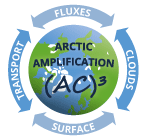
\includegraphics[height=8.0em]{logo_small-ac3.png}
    %\end{tabular}   
  }

%%%%%%%%%%%%%%%%%%%%%%%%%%%%%%%%%%%%%%%%%%%%%%%%%%%%%%%%%%%%%%%%%%%%%%%%%%%%%%
%%% Now define the boxes that make up the poster
%%%---------------------------------------------------------------------------
%%% Each box has a name and can be placed absolutely or relatively.
%%% The only inconvenience is that you can only specify a relative position 
%%% towards an already declared box. So if you have a box attached to the 
%%% bottom, one to the top and a third one which should be in between, you 
%%% have to specify the top and bottom boxes before you specify the middle 
%%% box.
%%%%%%%%%%%%%%%%%%%%%%%%%%%%%%%%%%%%%%%%%%%%%%%%%%%%%%%%%%%%%%%%%%%%%%%%%%%%%%
    %
    % A coloured circle useful as a bullet with an adjustably strong filling
    \newcommand{\colouredcircle}{%
      \vspace{1em}\tikz{\useasboundingbox (-0.2em,-0.32em) rectangle(0.2em,0.32em); \draw[draw=black,fill=lightblue,line width=0.03em] (0,0) circle(0.28em);}\hspace{0.8em}}

%%%%%%%%%%%%%%%%%%%%%%%%%%%%%%%%%%%%%%%%%%%%%%%%%%%%%%%%%%%%%%%%%%%%%%%%%%%%%%
  \headerbox{1.- Research Objectives}{name=objective,column=0,span=1,row=0}{
%%%%%%%%%%%%%%%%%%%%%%%%%%%%%%%%%%%%%%%%%%%%%%%%%%%%%%%%%%%%%%%%%%%%%%%%%%%%%%
The study focuses on the Western Arctic to address the following research questions:
\begin{itemize}
	\item How are macro- and microphysical cloud properties influenced by the presence of leads or polynyas?
	\item Are cloud radiative effects different during different sea ice conditions?
\end{itemize}

\begin{tabular*}{0.99\textwidth}[h!]{lc}
	\begin{minipage}{0.45\textwidth}
		\vspace{-3em}
	Location of the Atmospheric Radiation Measurement’s (ARM) North Slope of Alaska (NSA) site in Utqiagvik, Alaska.
	\end{minipage}
	&
	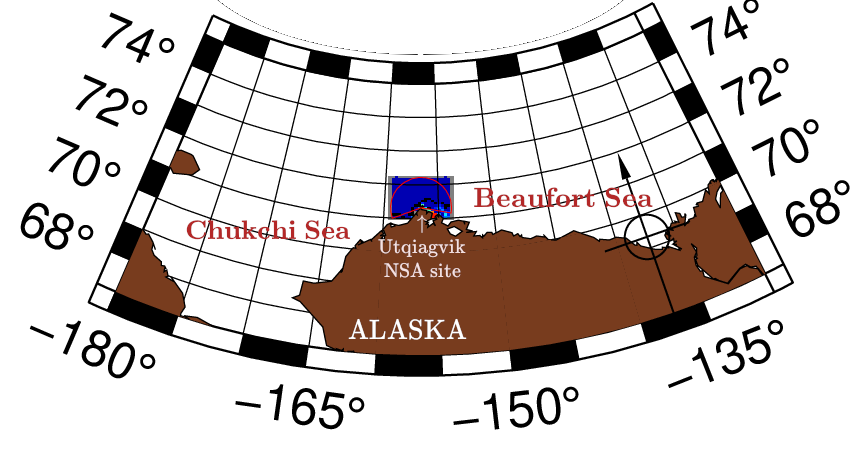
\includegraphics[scale=0.55]{NSA_SIC_100km.png}	
\end{tabular*}
\\
NSA provides long-term high-quality in-situ and remote-sensing observations for clouds and radiation. This study is concentrated on the Arctic winters from 2012 to 2020.	
  }
%%%%%%%%%%%%%%%%%%%%%%%%%%%%%%%%%%%%%%%%%%%%%%%%%%%%%%%%%%%%%%%%%%%%%%%%%%%%%%
\headerbox{2.- Coupling Sea Ice and Clouds}{name=retmethods,column=0,below=objective}{
%%%%%%%%%%%%%%%%%%%%%%%%%%%%%%%%%%%%%%%%%%%%%%%%%%%%%%%%%%%%%%%%%%%%%%%%%%%%%%
%\hspace{-2em}
Daily sea ice concentration (SIC) is primarily obtained from satellite retrievals provided by the University of Bremen [1], the following analysis is performed to couple sea ice conditions with cloud observations above NSA:

\colouredcircle SIC AMSR2 products is analyzed for a sector 50~km around the NSA site.\\
\begin{minipage}{0.9\textwidth}
	\begin{center}
		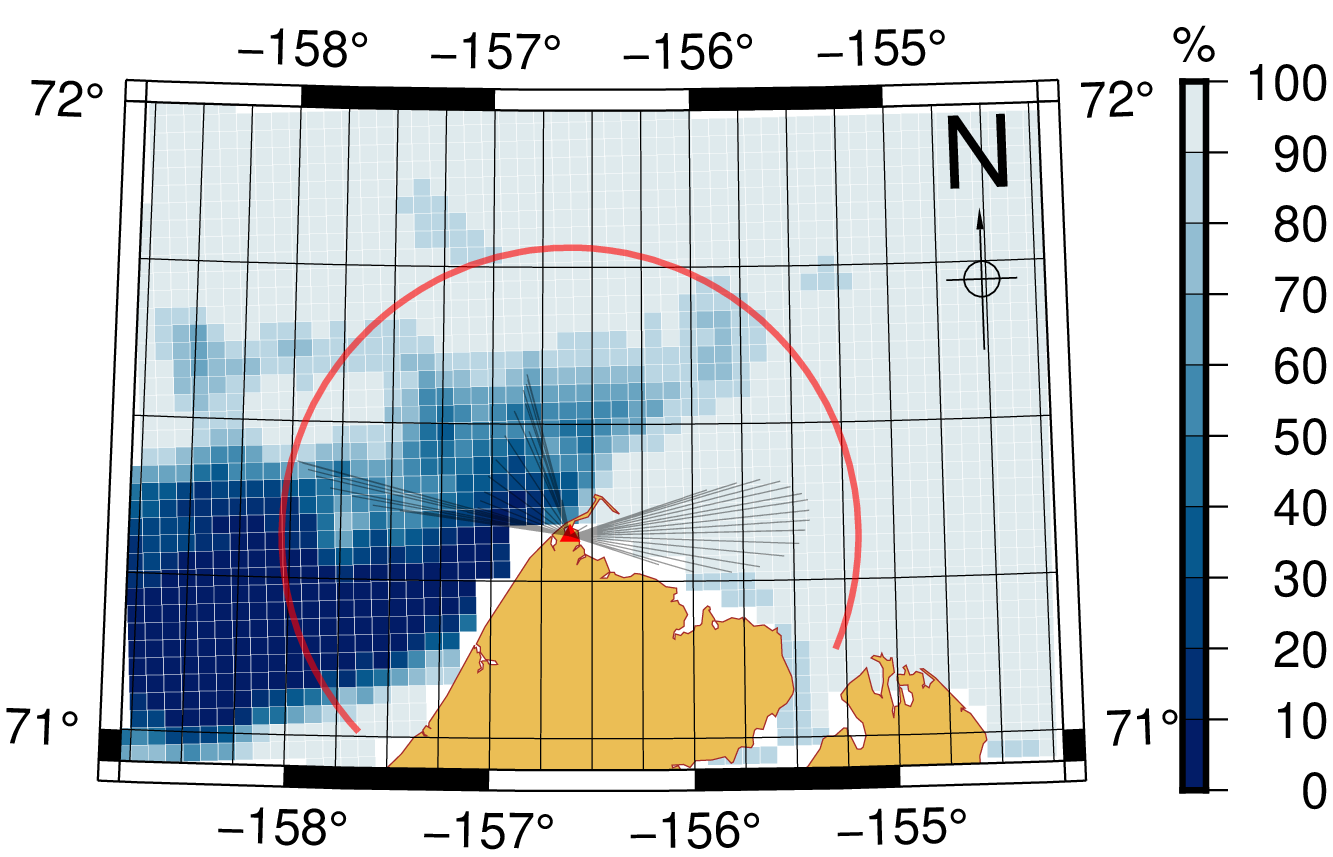
\includegraphics[width=.7\linewidth]{1411_NSA_SIC_wdir_2019-03-23.png}\\
		\emph{\small SIC (see colorbar) and wind direction at maximum water vapour transport (see red wind barb). Only SIC from those directions are considered.}
	\end{center}
\end{minipage}

\colouredcircle Sea ice - atmosphere coupling model\\
Gradient of water vapour transport ($\nabla_z WVT$) is calculated from humidity and radiosonde wind profiles. The direction of maximum transport (see grey lines in figure above) is used to relate SIC with zenith observations at NSA.
\begin{minipage}{0.9\textwidth}
	\begin{center}
		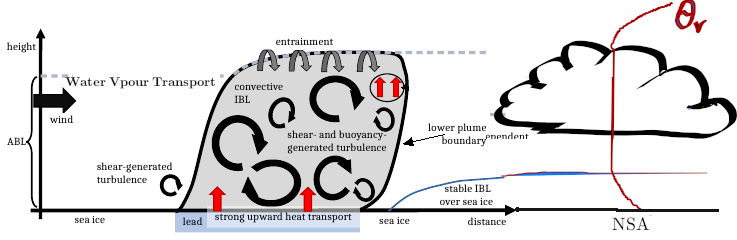
\includegraphics[width=.6\linewidth]{drawing_lead_cloud.png}\\
		\emph{\small Conceptual model for sea ice interaction with clouds.}
	\end{center}
\end{minipage}

The virtual potential temperature $\theta_v$ is analyzed to classify cases where the WVT is coupled or decoupled to the cloud.

\colouredcircle Cloud observation classification:\\
\begin{minipage}{0.9\textwidth}
\begin{center}
	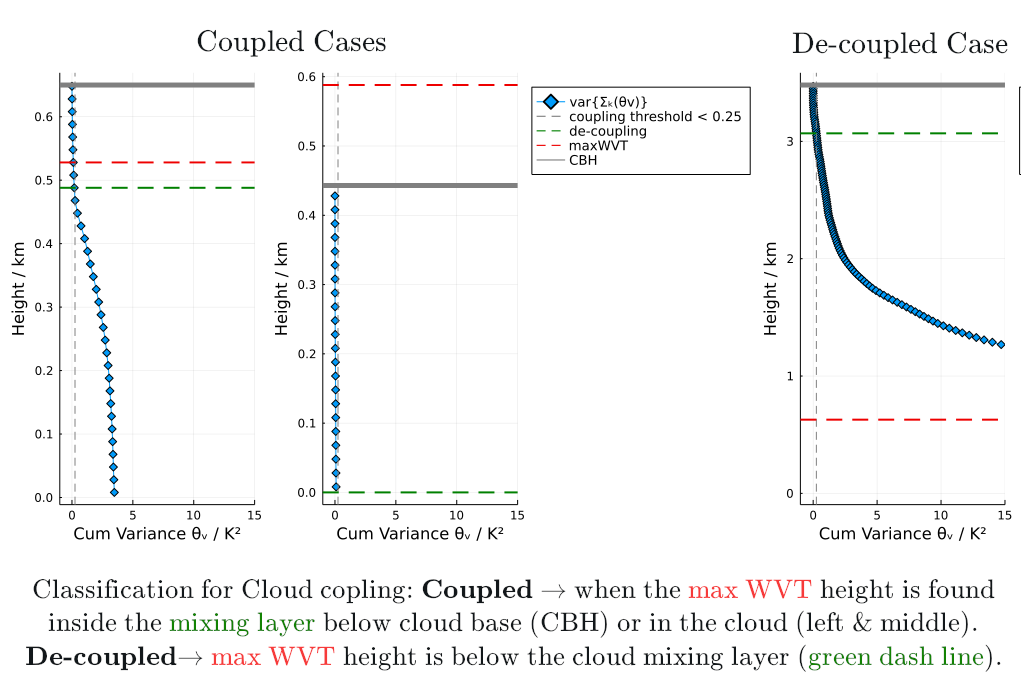
\includegraphics[width=0.6\linewidth]{images/coupling_no_coupling}\\
	\emph{\small Coupling / decoupling classification based on $\theta_v$ and location of maximum water vapour transport.}
\end{center}	
\end{minipage}


\colouredcircle Skin temperature is estimated considering SIC values:
\[
	T_{skin}(sic, T_s) = SST - SIC\times(SST~-~T_s)
\]
with $SST$ being sea surface temperature (assumed as 271.34~K), SIC from $0\dots1$, and $T_s$ the surface temperature derived from observations as:
\[
	T_s = \Big[ \frac{F_{lw}^{\downarrow} - (1-\varepsilon_s)F_{lw}^{\uparrow}}{\varepsilon_s~\sigma} \Big]^{\frac{1}{4}}
\]
being $F_{lw}^{\downarrow}$ and $F_{lw}^{\uparrow}$ down- and up-welling longwave fluxes measured at NSA. The surface emissivity $\varepsilon_s$ is considered 0.981 $\pm$ 5\%, which is a standard value for winter. \\
 
{\large The results are sorted based on the cloud-sea ice coupled/decoupled conditions. Statistics of LW net surface radiation and cloud radiative effects (CRE) are show in Section 3.}

} % end of box

%%%%%%%%%%%%%%%%%%%%%%%%%%%%%%%%%%%%%%%%%%%%%%%%%%%%%%%%%%%%%%%%%%%%%%%%%%%%%%
  \headerbox{3.- Results for coupled and decoupled cases}{name=results,column=1,row=0,span=2}{
%%%%%%%%%%%%%%%%%%%%%%%%%%%%%%%%%%%%%%%%%%%%%%%%%%%%%%%%%%%%%%%%%%%%%%%%%%%%%%
{\Large Surface longwave radiation fluxes observed at NSA are shown as function of several variables under the influence of sea ice conditions, e.g. liquid and ice water path (LWP, IWP), skin temperature based on SIC, and cloud radiating temperature:}\\
\vspace{+4.0em}
\begin{tabular}{c|c} %{@{}lcr@{}}
	\multicolumn{2}{l}{\vspace{+1em}\colouredcircle {\large Liquid water path \hfill}} \\
	\textbf{\Large COUPLED}	& \textbf{\Large DECOUPLED} \\
	\begin{minipage}{0.45\linewidth}
		\begin{center}
			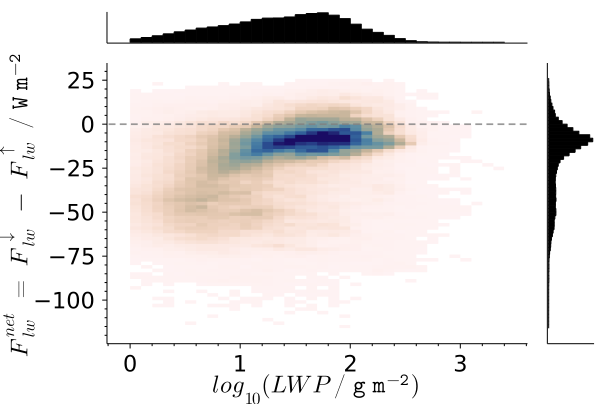
\includegraphics[width=.8\linewidth]{Fnet_vs_LWP_coupled.png}	
		\end{center}
	\end{minipage}
	&
	\begin{minipage}{0.45\linewidth}	
		\begin{center}             
			%\vspace{-0.2em}
			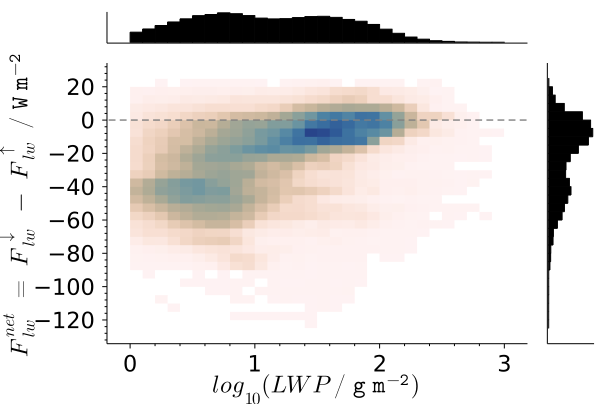
\includegraphics[width=.8\linewidth]{Fnet_vs_LWP_decoupled.png}
		\end{center}
	\end{minipage}\\
	\hline\\
	\multicolumn{2}{l}{\vspace{+1em}\colouredcircle {\large Net LW radiation \hfill}} \\
	\textbf{\Large COUPLED}	& \textbf{\Large DECOUPLED} \\
	\begin{minipage}{0.45\linewidth}
		\begin{center}
			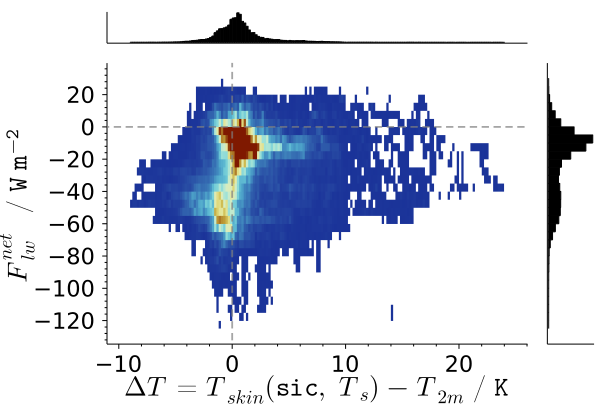
\includegraphics[width=.9\linewidth]{Fnet_vs_DeltaT_coupled.png}	
		\end{center}
	\end{minipage}
	&
	\begin{minipage}{0.45\linewidth}
		\begin{center}             
			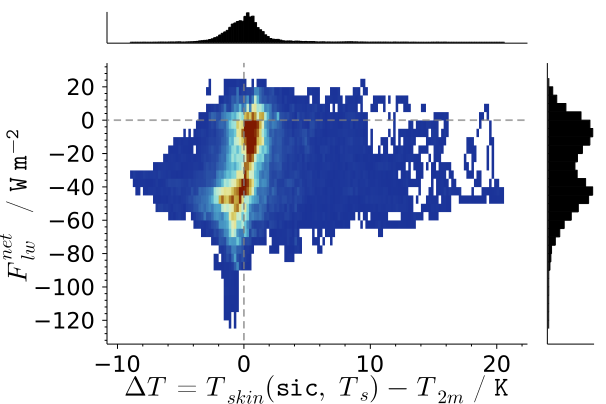
\includegraphics[width=.9\linewidth]{Fnet_vs_DeltaT_decoupled.png}
		\end{center}
	\end{minipage}\\
\end{tabular}\\

\begin{tabular}{@{}lcr@{}}
	\multicolumn{3}{l}{\vspace{+1em}\colouredcircle {\large Cloud Radiative Effect (CRE) for LW downwelling radiation \hfill}} \\
	\begin{minipage}{0.31\linewidth}
		\begin{center}             
			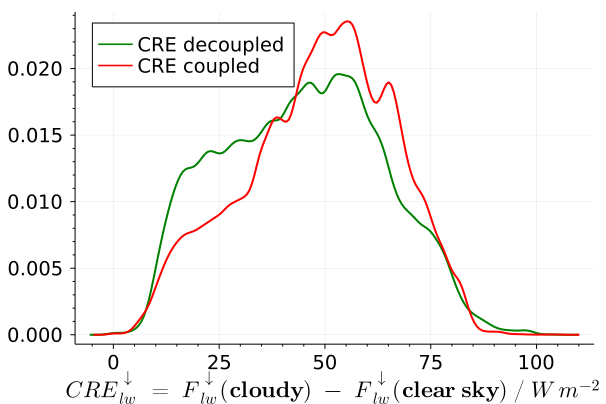
\includegraphics[width=.93\linewidth]{CRE_lw_dw.png}
		\end{center}
	\end{minipage} &
\begin{minipage}{0.31\linewidth}
	\begin{center}             
		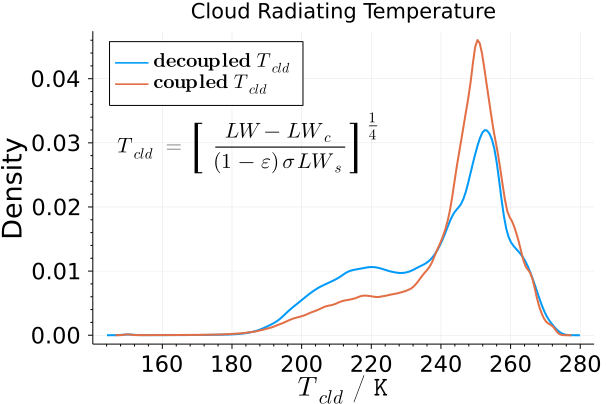
\includegraphics[width=.93\linewidth]{cloud_radiating_T.png}
	\end{center}
\end{minipage} &
\begin{minipage}{0.31\linewidth}
	\begin{center}             
		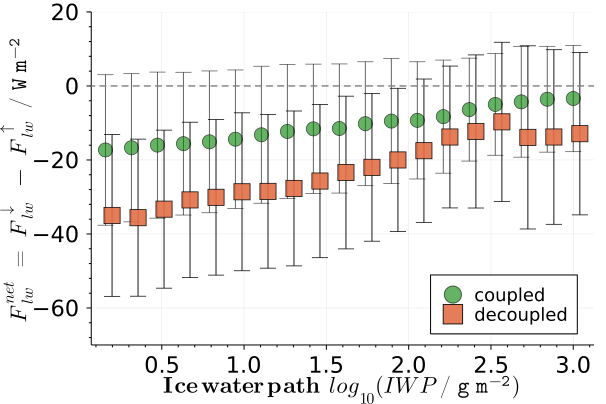
\includegraphics[width=.93\linewidth]{Fnet_vs_IWP_both.png}
	\end{center}
\end{minipage} \\
	\begin{minipage}{0.3\linewidth}
		PDF for CRE (cloudy - clear sky) for LW downwelling radiation shows a more frequent occurrence for cases when the clouds are coupled.
	\end{minipage} 
	&
	\begin{minipage}{0.3\linewidth}
		Cloud radiating temperature estimated from clear-sky LW ($LW_c$), fractional sky cover ($LW_c$), indicating similarly that warmer clouds are more frequent for coupled cases.
	\end{minipage}
	&
	\begin{minipage}{0.3\linewidth}
		LW net radiation as a function of observed ice water path (IWP).
	\end{minipage}
	\\		
\end{tabular}

CRE is calculated based on cloudy observations and corresponding clear-sky simulations following Long and Gaustad (2004) for shortwave radiation, and Brutsaert (1975) for longwave downwelling radiation. Clear sky calculation is a state-of-the-art value added product from ARM.
   
%\parbox[l]{0.8\linewidth}{   \vspace{-.5em}
%	{Some text here....}    
%}
}

%%%%%%%%%%%%%%%%%%%%%%%%%%%%%%%%%%%%%%%%%%%%%%%%%%%%%%%%%%%%%%%%%%%%%%%%%%%%%%
\headerbox{4.- Conclusions}{name=conclutions,column=1,span=2,below=results}{
  %%%%%%%%%%%%%%%%%%%%%%%%%%%%%%%%%%%%%%%%%%%%%%%%%%%%%%%%%%%%%%%%%%%%%%%%%%%%%%
{Ground-based radiation observations at the ARM site at the North Slope of Alaska (NSA) have been analyzed for the period of winters 2012 to 2020. The data has been classified into sea ice - cloud coupled/ decoupled cases. The results are consistent with previous findings regarding the effect of low sea ice concentration (e.g., due to the presence of leads or polynyas) on cloud micro- and macro-physical properties. Cloud properties like liquid and ice water path (LWP and IWP), cloud base height, and cloud geometrical thickness are also variables strongly influencing the surface radiation budget. Our results depict that a warming cloud effect on the surface is clearly enhanced by atmospheric thermodynamic and dynamic conditions which are coupled with the sea ice situation downwind.

So far only simulation of clear-sky for longwave downwelling radiation have been considered, in the future we will include complete clear-sky simulations following Kebell et al. (2020) for the central Arctic site Ny~Alesund, thus a better picture on CRE will be achieved.
}

% \sc (this make cool big font)!

}

%%%%%%%%%%%%%%%%%%%%%%%%%%%%%%%%%%%%%%%%%%%%%%%%%%%%%%%%%%%%%%%%%%%%%%%%%%%%%%
\headerbox{5.- References }{name=references,column=1, span=2, below=conclutions}{
%%%%%%%%%%%%%%%%%%%%%%%%%%%%%%%%%%%%%%%%%%%%%%%%%%%%%%%%%%%%%%%%%%%%%%%%%%%%%%
%\colouredcircle \hspace{2em}
\hspace{-2.4em}
\begin{minipage}{0.99\linewidth}
{\scriptsize
	\begin{enumerate}
		\item Inverse Methods for Atmospheric Sounding. Rodgers C.D. 2015. https://doi.org/10.1142/3171.
		\item \vspace{-0.6em} Bayesian Analysis in Inverse Problems, Fitzpatrick B.G. 1991. Inverse Problems 7, 675-702.
		\item \vspace{-0.6em} Instrument Operation \& Software guide, Issure 01/09, 2014. Radiometer Physics GmbH.
		\item \vspace{-0.6em} Wyoming Radiosonde Download Toolbox: https://github.com/pablosaa/WyoSonde
		\item \vspace{-0.6em} HATPRO Toolbox: https://github.com/pablosaa/HATPRO-DABINIO
		\item \vspace{-0.6em} Bayes Retrieval Toolbox: https://github.com/pablosaa/TroposProf
	\end{enumerate}
}	
\vspace{-0.6em}
\end{minipage}
	%\end{tabular}
	%\vspace{0.5em}
}
%%%%%%%%%%%%%%%%%%%%%%%%%%%%%%%%%%%%%%%%%%%%%%%%%%%%%%%%%%%%%%%%%%%%%%%%%%%%%%
\headerbox{6.- Acknowledges}{name=acknown,column=0, span=3, above=bottom}{
	%%%%%%%%%%%%%%%%%%%%%%%%%%%%%%%%%%%%%%%%%%%%%%%%%%%%%%%%%%%%%%%%%%%%%%%%%%%%%%
	{\small This work was supported by the DFG funded Transregio-project TR-172 "Arctic Amplification $(AC)^3$". The authors thanks the DOE ARM program for providing all data from the NSA site. Sea ice data is possible thanks to University of Bremen data repository and Dr. Gunnar Spreen for his collaboration. Cloud classification was performed by the open-source \emph{Cloudnetpy} algorithm by ACTRIS and FMI. }
}

\end{poster}

\end{document}

%%%%%%%%%%%%%%%%%%%%%%%%%%%%%%%%%%%%%%%%%%%%%%%%%%%%%%%%%%%%%%%%%%%%%%%%%%%%%%%
%\headerbox{6. References}{name=ref,column=4,above=bottom,span=1}{%
%	%%%%%%%%%%%%%%%%%%%%%%%%%%%%%%%%%%%%%%%%%%%%%%%%%%%%%%%%%%%%%%%%%%%%%%%%%%%%%%
%	\begin{tabular}{@{}l||c@{}}
%		\hspace{-1.2em}
%		\begin{minipage}{0.35\linewidth}
%			%\vspace{-9em}
%			{Virtual Observations (VO) are needed to test Data Assimilation schemes. In that sense, synthetic observations alike SMAP/SMOS satellites have been generated. For that task, satellite features like orbit, antenna pattern, foot-print, incidence angle have been taking into account.}\\
%			%{\color{yellow} The statistics comprise of pixels within the Neckar catchment D4 after antenna pattern and real-orbit considerations. TOP PANEL: descending-orbit; BOTTOM PANEL: ascending-orbit.}
%			\vspace{-1.5em}
%			\begin{center}
%				%\includegraphics[width=.45\linewidth,height=115px]{img_lwc_10:30.png} &
%				\includegraphics[width=.5\linewidth]{AntennaPattern.png}
%			\end{center}
%			The above antenna pattern is a proxy for SMAP specifications, with a 3dB FWHM FOV of 2.4° and footprint of 36km. The pattern is applied to the high-resolution D4 simulations and SMAP Passive L2C\_TB\_PA synthetic data is generated.
%		\end{minipage}
%		%\vspace{-4em}
%		&
%		\begin{minipage}{0.6\linewidth}
%			\vspace{-0.1em}
%			\begin{center}
%				The synthetic observations are rendered according to the EASE-grid corresponding for the D4 catchment geo-locations i.e. 36km grid a like SMAP L2 data.\\
%				%     \hspace{-5em}
%				\includegraphics[scale=.5]{TBHcube_CLM_SAT.png}\\
%				{\color{red} SMAP virtual observations:} in the above figure the bottom-plane corresponds to TB high-res (206x234), while the top-plane the TB at EASE-grid D4 resolution (6x6). 
%				
%				%\includegraphics[width=.95\linewidth]{cmem_smosDA_BoxP2013.png}
%				%      \\
%				%      {\vspace{-2px} \sc \small
%				%      The Optical thicknesses retrieved from. 
%				%      }
%			\end{center}
%			%\vspace{8cm}
%		\end{minipage}
%	\end{tabular}\\
%	\begin{minipage}{0.98\linewidth}
%		\vspace{+0.2em}
%		\centering
%		\includegraphics[width=0.85\linewidth,height=7cm]{summer_TBclmSmap_ts.png}
%	\end{minipage}
%}
%%%%%%%%%%%%%%%%%%%%%%%%%%%%%%%%%%%%%%%%%%%%%%%%%%%%%%%%%%%%%%%%%%%%%%%%%%%%%%%
%\headerbox{7. Soil Moisture Bias in CLM}{name=clmbias,column=2,below=cmemout,span=2}{%
%	%%%%%%%%%%%%%%%%%%%%%%%%%%%%%%%%%%%%%%%%%%%%%%%%%%%%%%%%%%%%%%%%%%%%%%%%%%%%%%
%	\begin{tabular}{@{}c||c@{}}
%		\begin{minipage}{0.5\linewidth}
%			%\vspace{-9em}
%			{CLM shows large values for soil moisture, which leads to huge bias on TB. CDF matching method used to correct SM with real SMAP retrievals as reference (left plot). To understand the effects on TB by decreasing SM, various factors $\eta$ has been used to fit a curve (rigth plot)}\\
%			\vspace{-1.2em}
%			\begin{center}
%				\includegraphics[width=.48\linewidth]{cdfSM_clm_smap.png} \hspace{0.01cm}
%				\includegraphics[width=.49\linewidth]{deltaTB_fSM.png}
%			\end{center}
%			It has been found that CLM soil moisture values are in average 45\% ($\eta$=0.55) higher than SMAP retrievals for 1 year comparison. Then the factor $\eta$ is used to calibrate soil moisture to input the forward operator.
%		\end{minipage}
%		&
%		\begin{minipage}{0.44\linewidth}
%			{After calibration for Soil Moisture, the TB bias is partially reduced but not completely: The following plots are biases in a pixel-to-pixel comparison from VR and SMAP data after an average catchment bias is subtracted. The color of the EASE-grid pixel indicates residual bias and the value inside every circle is its respective ubRMSE.}\\
%			\vspace{-.2em}
%			\begin{center}
%				\includegraphics[width=.495\linewidth]{DIFF_TBH_VRD4_SMAP.png}\hspace{0.01cm}
%				\includegraphics[width=.495\linewidth]{DIFF_TBV_VRD4_SMAP.png}
%			\end{center}
%		\end{minipage}\\
%		\hline
%	\end{tabular}\\
%	
%	\begin{minipage}{0.95\linewidth}
%		\vspace{+.7em}
%		{\color{green} CONCLUSIONS:} 
%		It has been found that Bayesian inversion is able to more accurately reproduce the profiles vertical structure in contrast to the firmware retrieval methods. This is primary true for the case of humidity and temperature profiles.
%		%Moreover cases of synergy with a wind profiler are applied to the Bayesian scheme producing a consistent temperature, humidity and lower atmosphere wind shears simultaneously.
%		
%		The presented methodology for ground-based atmospheric profiling produces results resembling observations by radiosondes when a suitable a-priori dataset is used. Moreover the open source tools needed to produce the a-priori dataset for the Bayesian inversion is available on to be used by the scientific community.
%	\end{minipage}
%}
